\documentclass[11pt,a4paper]{article}

% ------------------------------------------------------------------
% Packages
% ------------------------------------------------------------------
\usepackage[T1]{fontenc}
\usepackage{lmodern}
\usepackage[a4paper,left=1.8cm,right=1.8cm,top=2cm,bottom=2cm]{geometry}
\usepackage{microtype}
\usepackage{needspace}
\usepackage{enumitem}
\usepackage{longtable}
\usepackage[compact]{titlesec}
\usepackage{amsmath,amssymb}
\usepackage{graphicx}
\usepackage{booktabs}
\usepackage{xcolor}
\usepackage{listings}
\usepackage{caption}
\usepackage{float}
\usepackage{setspace}
\usepackage[colorlinks=true,linkcolor=blue!50!black,citecolor=blue!50!black,urlcolor=blue!50!black]{hyperref}

\graphicspath{{figures/}}
\setstretch{1.05}
\setlength{\parindent}{0pt}
\setlength{\parskip}{0.4em}
\setlength{\emergencystretch}{3em}
\widowpenalty=10000
\clubpenalty=10000
\setlength{\abovedisplayskip}{4pt}
\setlength{\belowdisplayskip}{4pt}
\renewcommand{\arraystretch}{1.15}
\raggedbottom
\setlist{itemsep=2pt,topsep=3pt,parsep=0pt}
\captionsetup{font=small,labelfont=bf}

% ------------------------------------------------------------------
% Macros
% ------------------------------------------------------------------
\newcommand{\bx}{\mathbf{x}}
\newcommand{\br}{\mathbf{r}}
\newcommand{\bv}{\mathbf{v}}
\newcommand{\bz}{\mathbf{z}}
\newcommand{\by}{\mathbf{y}}
\newcommand{\bu}{\mathbf{u}}
\newcommand{\ba}{\mathbf{a}}
\newcommand{\bd}{\mathbf{d}}
\newcommand{\bF}{\mathbf{F}}
\newcommand{\bH}{\mathbf{H}}
\newcommand{\bP}{\mathbf{P}}
\newcommand{\bQ}{\mathbf{Q}}
\newcommand{\bR}{\mathbf{R}}
\newcommand{\bK}{\mathbf{K}}
\newcommand{\bS}{\mathbf{S}}
\newcommand{\bI}{\mathbf{I}}
\newcommand{\bzero}{\mathbf{0}}
\newcommand{\T}{^{\top}}

% ------------------------------------------------------------------
% MATLAB listing style
% ------------------------------------------------------------------
\lstset{
  language=Matlab,
  basicstyle=\ttfamily\fontsize{8}{9.6}\selectfont,
  keywordstyle=\color{blue},
  commentstyle=\color{green!45!black},
  stringstyle=\color{purple},
  numbers=left,
  numberstyle=\tiny\color{gray},
  numbersep=6pt,
  frame=single,
  rulecolor=\color{black!30},
  breaklines=true,
  showstringspaces=false,
  tabsize=4,
  columns=fullflexible,
  keepspaces=true,
  captionpos=b,
  aboveskip=6pt,
  belowskip=4pt
}

\begin{document}

% ==================================================================
% Title page
% ==================================================================
\begin{titlepage}
\centering
\vspace*{0.5cm}

\includegraphics[width=4.3cm]{uom_logo.png}\\[1.6cm]

\includegraphics[width=5.8cm]{entc_logo.png}\\[1.8cm]

{\LARGE\bfseries Satellite Orbit Determination from\\[0.2cm] Ground-Station Range and Range-Rate\\[0.2cm] Measurements\par}
\vspace{0.5cm}
{\large Mini Project: Extended Kalman Filter\par}
\vspace{0.8cm}
{\large EN4594 \textemdash{} Autonomous Systems\par}

\vspace{1.6cm}
\begin{tabular}{@{}l@{\hspace{1.2cm}}l@{}}
  \textbf{Name:}      & PRAVEEN V.V.J. \\
  \textbf{Index No:}  & 220491B \\
\end{tabular}

\vfill
\textbf{Date:} \the\day/\the\month/\the\year
\vspace{1cm}
\end{titlepage}

\setcounter{tocdepth}{2}
\tableofcontents
\newpage
\listoffigures
\listoftables
\newpage

% ==================================================================
% 1 Introduction
% ==================================================================
\section{Introduction}

\subsection{Background}
Knowing where a satellite is, and where it will be, is the basis of almost every space operation: pointing antennas, planning manoeuvres, avoiding collisions and combining payload data with location.
This task is called orbit determination.
In practice the satellite state cannot be observed directly. Instead, ground stations measure quantities that depend on the state, such as the distance to the satellite (range) and how fast that distance is changing (range-rate, obtained from the Doppler shift). These measurements are noisy, and they are available only while the satellite is above the station's horizon.
A state estimator is therefore needed to combine an imperfect dynamics model with noisy, intermittent measurements.

\subsection{Objective}
The aim of this mini project is to implement a state estimation filter for a specific application and to demonstrate its effectiveness, as required by the assignment.
The chosen combination is:
\begin{itemize}
  \item \textbf{Filter:} Extended Kalman Filter (EKF);
  \item \textbf{Application:} satellite orbit determination from ground-station range and range-rate measurements.
\end{itemize}
The specific goals are to
\begin{enumerate}
  \item derive the dynamics and measurement models and their Jacobians;
  \item implement the EKF in MATLAB;
  \item evaluate it in simulation, using plots and statistical consistency tests (NEES and NIS, explained in Section~\ref{sec:checks});
  \item explore its capabilities and limitations by changing the scenario and the filter parameters.
\end{enumerate}

\subsection{Why an Extended Kalman Filter?}
The standard Kalman filter is optimal for linear systems with Gaussian noise. Both parts of this problem are nonlinear:
\begin{itemize}
  \item the gravitational acceleration $-\mu\,\br/\|\br\|^3$ is nonlinear in the position;
  \item the range $\rho=\|\br-\br_s\|$ and range-rate $\dot\rho$ are nonlinear in the state.
\end{itemize}
As presented in the lectures (Gaussian Filters III), the EKF handles such systems by linearising the state-transition and measurement models about the current estimate with a first-order Taylor expansion, and then applying the Kalman filter equations.
It is computationally cheap and it is the most widely used nonlinear estimator, which makes it well suited to a six-dimensional state that is propagated for many hours.
A particle filter could also represent nonlinear problems, but it needs a very large number of particles in six dimensions when the measurements are as accurate as here, so it is far more expensive for little benefit.
The orbit problem is also only mildly nonlinear over the time spans of interest, which is the situation where the EKF works well.

\subsection{How the EKF is checked: NEES and NIS}
\label{sec:checks}
A filter should be accurate, but it should also be honest about how accurate it is. The EKF produces a covariance matrix $\bP$ that states how uncertain it believes its own estimate to be. To check that this claim is true, two standard consistency tests are used throughout the results (Section~4):
\begin{itemize}
  \item \textbf{NEES} (Normalised Estimation Error Squared) compares the actual error of the estimate with the uncertainty the filter claims. It needs the true state, so it can be used in simulation only. For a consistent filter its average is about 6 (the number of states). Values much larger than this mean the filter is overconfident; values much smaller mean it is too cautious.
  \item \textbf{NIS} (Normalised Innovation Squared) compares each new measurement with the prediction the filter made before seeing it, scaled by the predicted uncertainty. It needs no true state, so it can also be used with real data. For a consistent filter its average is about 2 (one range and one range-rate value per measurement).
\end{itemize}
Together with the $\pm3\sigma$ error bounds and the normalised innovations, these tests show whether the EKF is correctly tuned. Their exact definitions are given in Section~\ref{sec:metrics}.

\subsection{Report outline}
Section~2 gives the theory: the models, the Jacobian derivations and the filter equations.
Section~3 describes the simulation and the MATLAB implementation.
Section~4 presents the results, and Section~5 discusses them and the limitations of the method.
Section~6 concludes. The complete MATLAB code is in Appendix~A.

\subsection{Key terms}
Table~\ref{tab:terms} explains in plain words the main terms used in this report.

\begin{longtable}{p{0.22\textwidth}p{0.72\textwidth}}
\caption{Key terms used in this report.}\label{tab:terms}\\
\toprule
\textbf{Term} & \textbf{Meaning in plain words} \\
\midrule
\endfirsthead
\toprule
\textbf{Term} & \textbf{Meaning in plain words (continued)} \\
\midrule
\endhead
\bottomrule
\endlastfoot
State & The numbers that describe the satellite: its position ($x,y,z$) and its velocity (three more numbers), six in total. \\
ECI & Earth-Centred Inertial frame. Its origin is the centre of the Earth, and it does not rotate with the Earth. Newton's laws, and therefore the satellite's orbit, are written in this frame. \\
ECEF & Earth-Centred, Earth-Fixed frame. Its origin is also the centre of the Earth, but it rotates with the Earth ($z$ axis through the North Pole, $x$ axis towards 0$^\circ$ longitude on the equator). A ground station has fixed coordinates here. \\
Range, range-rate & Range is the straight-line distance from a ground station to the satellite. Range-rate is how fast that distance is changing (positive when the satellite moves away), measured from the Doppler shift of the radio signal. \\
Elevation, pass & Elevation is the angle of the satellite above the local horizon. A pass is a period when the satellite is high enough (here above $10^\circ$) for the station to take measurements. \\
$J_2$ & The main effect of the Earth being slightly flattened (it bulges at the equator) on a satellite's orbit. \\
Drag & A small braking force from the thin upper atmosphere. It is included in the simulated truth but not in the filter's model. \\
Jacobian & A matrix of partial derivatives. It is the straight-line (linear) approximation of a nonlinear function around the current estimate, which is what the EKF uses. \\
Covariance $\bP$ & A matrix that describes how uncertain the filter believes its estimate is. \\
Process noise $\bQ$ & An allowance for effects the filter's model does not include (such as drag), which makes the uncertainty grow between measurements. \\
Innovation & The difference between a real measurement and the value the filter predicted for it: how much the measurement surprised the filter. \\
RMS error & Root mean square error: the typical size of the error over a period of time. \\
$\sigma$, $3\sigma$ bound & $\sigma$ is one standard deviation (the filter's claimed uncertainty). About 99.7\% of errors should stay inside $\pm3\sigma$. \\
\end{longtable}


% ==================================================================
% 2 Methodology
% ==================================================================
\clearpage
\section{Methodology}

\subsection{Problem formulation}
The state is the satellite position and velocity in an Earth-Centred Inertial (ECI) frame. This is a coordinate frame with its origin at the centre of the Earth that does not rotate with the Earth, which is the natural frame for writing Newton's laws and the satellite's orbit. (The ground stations are described in a second frame, ECEF, introduced in Section~\ref{sec:station}.) The state is
\begin{equation}
  \bx = \begin{bmatrix}\br\\ \bv\end{bmatrix}\in\mathbb{R}^6 ,
  \qquad \br=[x,\,y,\,z]\T,\quad \bv=[\dot x,\,\dot y,\,\dot z]\T .
\end{equation}
Units are kilometres and seconds throughout.
The filter works in discrete time with steps of $\Delta t=10$~s. At each step $k$ it holds an estimate $\hat\bx_k$ and a covariance $\bP_k$.
The system is described by
\begin{align}
  \bx_k &= \phi(\bx_{k-1}) + \mathbf{w}_k, & \mathbf{w}_k &\sim \mathcal{N}(\bzero,\bQ_k), \\
  \bz_k &= h(\bx_k) + \mathbf{v}_k,        & \mathbf{v}_k &\sim \mathcal{N}(\bzero,\bR),
\end{align}
where $\phi$ is the orbit propagation over one step, $h$ is the measurement model, $\bQ_k$ is the process-noise covariance and $\bR$ is the measurement-noise covariance.

\subsection{Orbital dynamics}
\label{sec:dyn}
The continuous-time dynamics are
\begin{equation}
  \dot\br = \bv, \qquad \dot\bv = \ba(\br) = \ba_{\text{2B}} + \ba_{J_2}.
\end{equation}
The first term is point-mass (two-body) gravity,
\begin{equation}
  \ba_{\text{2B}} = -\frac{\mu}{r^{3}}\,\br, \qquad r=\|\br\|,
\end{equation}
with $\mu=398600.4418$~km$^3$/s$^2$.
The second term is the perturbation caused by the Earth's equatorial bulge, which is by far the largest perturbation for a low orbit:
\begin{equation}
  \ba_{J_2} = -\frac{3}{2}\,J_2\,\frac{\mu R_e^{2}}{r^{5}}
  \begin{bmatrix}
    x\,\bigl(1-5z^2/r^2\bigr)\\[2pt]
    y\,\bigl(1-5z^2/r^2\bigr)\\[2pt]
    z\,\bigl(3-5z^2/r^2\bigr)
  \end{bmatrix},
\end{equation}
with $J_2=1.08263\times10^{-3}$ and $R_e=6378.137$~km.
At this altitude (about 620~km) $\ba_{J_2}$ is about $10^{-5}$~km/s$^2$, roughly $10^{-3}$ of the main gravity term. This looks small, but integrated over a gap of 1.5~hours it moves the satellite by an amount of the order of $\tfrac12(10^{-5})(5400)^2\approx 150$~km, so it cannot be ignored (see Section~\ref{sec:j2study}).

\subsection{Measurement model}
\subsubsection{Station kinematics}
\label{sec:station}
Ground stations are easiest to describe in the Earth-Centred, Earth-Fixed (ECEF) frame. Like ECI, its origin is the centre of the Earth, but it rotates with the Earth: the $z$ axis points through the North Pole and the $x$ axis points to 0$^\circ$ longitude on the equator. A station on the ground therefore has constant ECEF coordinates. A station with geodetic latitude $\varphi$, longitude $\lambda$ and altitude $h_s$ has ECEF position (WGS-84 ellipsoid)
\begin{equation}
  \br_s^{\text{ECEF}} =
  \begin{bmatrix}
    (N+h_s)\cos\varphi\cos\lambda\\
    (N+h_s)\cos\varphi\sin\lambda\\
    \bigl(N(1-e^2)+h_s\bigr)\sin\varphi
  \end{bmatrix},
  \qquad N=\frac{R_e}{\sqrt{1-e^2\sin^2\varphi}} .
\end{equation}
The satellite state is in ECI, so the station position must be converted from ECEF to ECI. Because the Earth rotates at $\omega_e=7.2921159\times10^{-5}$~rad/s, the station moves in the inertial frame:
\begin{equation}
  \br_s(t)=\mathbf{R}_3(\omega_e t)\,\br_s^{\text{ECEF}},\qquad
  \bv_s(t)=\boldsymbol{\omega}_e\times\br_s(t),\qquad
  \boldsymbol{\omega}_e=[0,\,0,\,\omega_e]\T ,
\end{equation}
where $\mathbf{R}_3$ is a rotation about the $z$ axis. (Precession and nutation are neglected; the Greenwich angle is zero at $t=0$.)

\subsubsection{Range and range-rate}
Let $\bd=\br-\br_s$ be the station-to-satellite vector, $\rho=\|\bd\|$, $\bu=\bd/\rho$ the line-of-sight unit vector and $\delta\bv=\bv-\bv_s$ the relative velocity. The measurement vector is
\begin{equation}
  \bz = h(\bx) =
  \begin{bmatrix}\rho\\ \dot\rho\end{bmatrix}
  =
  \begin{bmatrix}\|\bd\|\\[2pt] \bu\T\,\delta\bv\end{bmatrix}.
\end{equation}
A measurement is available only when the satellite is above a minimum elevation of $10^\circ$, i.e.\ when $\arcsin(\bd\cdot\hat{\mathbf{n}}/\rho)\ge10^\circ$, where $\hat{\mathbf n}$ is the local vertical at the station.

\subsubsection{Measurement Jacobian}
The EKF needs $\bH=\partial h/\partial\bx$. The derivation is short.
For the range,
\begin{equation}
  \frac{\partial\rho}{\partial\br}=\frac{\bd\T}{\rho}=\bu\T,\qquad
  \frac{\partial\rho}{\partial\bv}=\bzero\T .
\end{equation}
For the range-rate $\dot\rho=\bu\T\delta\bv$ we use $\partial\bu/\partial\br=(\bI-\bu\bu\T)/\rho$, which gives
\begin{equation}
  \frac{\partial\dot\rho}{\partial\br}
  =\frac{\delta\bv\T(\bI-\bu\bu\T)}{\rho}
  =\frac{(\delta\bv-\dot\rho\,\bu)\T}{\rho},
  \qquad
  \frac{\partial\dot\rho}{\partial\bv}=\bu\T .
\end{equation}
Therefore
\begin{equation}
  \bH=
  \begin{bmatrix}
    \bu\T & \bzero\T\\[3pt]
    \dfrac{(\delta\bv-\dot\rho\,\bu)\T}{\rho} & \bu\T
  \end{bmatrix}\in\mathbb{R}^{2\times6}.
  \label{eq:H}
\end{equation}
The measurement noise has $\sigma_\rho=10$~m and $\sigma_{\dot\rho}=1$~mm/s, so $\bR=\mathrm{diag}(\sigma_\rho^2,\sigma_{\dot\rho}^2)$.

\subsection{Linearisation of the dynamics: state-transition matrix}
Writing the dynamics as $\dot\bx=f(\bx)$, the Jacobian is
\begin{equation}
  \mathbf{A}=\frac{\partial f}{\partial\bx}=
  \begin{bmatrix}\bzero & \bI\\ \mathbf{G} & \bzero\end{bmatrix},
  \qquad \mathbf{G}=\frac{\partial\ba}{\partial\br}.
\end{equation}
For the two-body term the gravity gradient is available in closed form,
\begin{equation}
  \mathbf{G}_{\text{2B}}=\frac{\mu}{r^3}\left(3\,\hat{\br}\hat{\br}\T-\bI\right),
\end{equation}
and the $J_2$ part of $\mathbf{G}$ is obtained by central finite differences of $\ba_{J_2}$ in the code, which keeps the implementation compact and easy to change.
The Jacobian that the EKF needs for the prediction step is the state-transition matrix $\bF_k=\boldsymbol{\Phi}(t_k,t_{k-1})$ of the linearised system, which is obtained by integrating the variational equations together with the state:
\begin{equation}
  \dot{\boldsymbol\Phi}=\mathbf{A}\,\boldsymbol\Phi,\qquad \boldsymbol\Phi(t_{k-1},t_{k-1})=\bI .
  \label{eq:stm}
\end{equation}
The 6 state equations and the 36 equations for $\boldsymbol\Phi$ are integrated together with a fourth-order Runge--Kutta (RK4) scheme.

\subsection{Process noise}
No model is perfect: drag, higher-order gravity terms, solar radiation pressure and third-body forces are not modelled. These errors are represented by white acceleration noise with power spectral density $q$ (km$^2$/s$^3$), the main tuning parameter (Section~\ref{sec:qstudy}). Over one step it gives
\begin{equation}
  \bQ_k = q
  \begin{bmatrix}
    \tfrac{\Delta t^3}{3}\bI & \tfrac{\Delta t^2}{2}\bI\\[3pt]
    \tfrac{\Delta t^2}{2}\bI & \Delta t\,\bI
  \end{bmatrix}.
\end{equation}
\subsection{The Extended Kalman Filter}
The EKF is the Kalman filter with the linear models replaced by their Jacobians. The state-transition function is linearised about the previous estimate and the measurement function about the predicted estimate. Because the Jacobians depend on these estimates, they must be recomputed at every step and cannot be calculated in advance. The orbit is driven by gravity only, so there is no control input. Table~\ref{tab:notation} lists the symbols used in the equations below.

\begin{table}[!htbp]
\centering
\caption{Notation used in the EKF equations.}
\label{tab:notation}
\begin{tabular}{lc}
\toprule
\textbf{Quantity} & \textbf{Symbol} \\
\midrule
Estimated state (mean), predicted & $\hat\bx_k$, $\bar\bx_k$ \\
Covariance, predicted & $\hat\bP_k$, $\bar\bP_k$ \\
State-transition function & $\phi(\cdot)$ \\
Jacobian of the state transition & $\bF_k=\boldsymbol\Phi$ \\
Measurement function, Jacobian & $h$, $\bH_k$ \\
Process-noise covariance & $\bQ_k$ \\
Measurement-noise covariance & $\bR$ \\
Kalman gain & $\bK_k$ \\
Time index & $k$ \\
\bottomrule
\end{tabular}
\end{table}

\paragraph{Prediction.}
\begin{align}
  \bar{\bx}_k &= \phi(\hat\bx_{k-1}) \quad\text{(RK4 integration of the dynamics)}, \\
  \bF_k &= \boldsymbol\Phi(t_k,t_{k-1}) \quad\text{from \eqref{eq:stm}}, \\
  \bar{\bP}_k &= \bF_k\,\hat{\bP}_{k-1}\,\bF_k\T+\bQ_k .
\end{align}

\paragraph{Correction} (for each station with a measurement $\bz_k$):
\begin{align}
  \bH_k &= \bH(\bar\bx_k)\quad\text{from \eqref{eq:H}}, \\
  \by_k &= \bz_k-h(\bar\bx_k) &&\text{(innovation)}, \\
  \bS_k &= \bH_k\bar{\bP}_k\bH_k\T+\bR &&\text{(innovation covariance)}, \\
  \bK_k &= \bar{\bP}_k\bH_k\T\bS_k^{-1} &&\text{(Kalman gain)}, \\
  \hat\bx_k &= \bar\bx_k+\bK_k\by_k, \\
  \hat{\bP}_k &= (\bI-\bK_k\bH_k)\,\bar{\bP}_k\,(\bI-\bK_k\bH_k)\T+\bK_k\bR\bK_k\T .
  \label{eq:joseph}
\end{align}
Equation~\eqref{eq:joseph} is the Joseph form of the covariance update. It equals $(\bI-\bK_k\bH_k)\bar\bP_k$ algebraically but keeps $\hat\bP$ symmetric and positive definite despite rounding errors, which matters because the covariance spans kilometres to metres.

\paragraph{Several stations.}
When more than one station sees the satellite at the same time, the correction step is repeated once per station, using each station's own $\bH$ and the already-updated $\hat\bx$ and $\hat\bP$. All stations are sampled on the same 10~s time grid as the filter, so no interpolation between timestamps is needed. Between passes only the prediction step runs.

\subsection{Performance and consistency metrics}
\label{sec:metrics}
Standard consistency tests for Kalman filters are used. Since the truth is known in simulation, the estimation error is $\mathbf{e}_k=\hat\bx_k-\bx_k^{\text{true}}$. The following measures are used.
\begin{itemize}
  \item \textbf{RMS position and velocity error}, computed after a 2-hour start-up period.
  \item \textbf{$3\sigma$ bounds:} the error should stay inside $\pm3\sqrt{P_{ii}}$ for about 99.7\% of the time.
  \item \textbf{NEES} (normalised estimation error squared): $\epsilon_k=\mathbf{e}_k\T\hat\bP_k^{-1}\mathbf{e}_k$. For a consistent filter, $\epsilon_k\sim\chi^2_6$, with mean 6 and 95\% bounds $[1.237,\,14.449]$. Values far below the range mean the filter is pessimistic; values far above mean it is overconfident.
  \item \textbf{NIS} (normalised innovation squared): $\nu_k=\by_k\T\bS_k^{-1}\by_k\sim\chi^2_2$, with mean 2 and 95\% bounds $[0.0506,\,7.378]$. NIS needs no truth, so it also works on real data. The normalised innovations $y_i/\sqrt{S_{ii}}$ should be zero-mean with unit variance.
\end{itemize}

% ==================================================================
% 3 Implementation
% ==================================================================
\clearpage
\section{Implementation}

\subsection{Simulation scenario}
All settings are collected in \texttt{default\_config.m}. The scenario is summarised in Table~\ref{tab:scenario}.

\begin{table}[H]
\centering
\caption{Simulation scenario and filter settings.}
\label{tab:scenario}
\begin{tabular}{lp{0.72\textwidth}}
\toprule
\textbf{Item} & \textbf{Value} \\
\midrule
Orbit & $a=7000$~km, $e=0.001$, $i=98^\circ$ (sun-synchronous LEO), $\Omega=40^\circ$, $\omega=0^\circ$, $\nu_0=0^\circ$ \\
Orbital period & 97.1 minutes \\
Duration, time step & 24~h, $\Delta t=10$~s (8641 epochs) \\
Truth dynamics & two-body $+\,J_2\,+$ constant drag $10^{-10}$~km/s$^2$, integrated with \texttt{ode45} (RelTol $10^{-10}$) \\
Filter dynamics & two-body $+\,J_2$, integrated with RK4 (drag is not modelled) \\
Ground stations & Moratuwa (Sri Lanka), London (UK), New York (USA), Tokyo (Japan), Sydney (Australia), Moscow (Russia) \\
Minimum elevation & $10^\circ$ \\
Measurements & range ($\sigma=10$~m), range-rate ($\sigma=1$~mm/s) \\
Initial covariance $\bP_0$ & $\mathrm{diag}\bigl((1\,\text{km})^2\times3,\;(1\,\text{m/s})^2\times3\bigr)$ \\
Initial estimate & truth plus a random error drawn from $\bP_0$ (0.55~km, 2.69~m/s) \\
Process noise $q$ & $10^{-16}$~km$^2$/s$^3$ \\
Random seed & 1 (fixed, so results are reproducible) \\
\bottomrule
\end{tabular}
\end{table}

The truth is produced by a different integrator (\texttt{ode45}) than the one used inside the filter (RK4), and it contains a drag force that the filter does not know about. This avoids the ``inverse crime'' of testing a filter on data generated by exactly the same model, and it gives the process noise $\bQ$ a real purpose.
The six stations are well-known cities spread over the globe (Figure~\ref{fig:track}). Moratuwa is close to the equator, while London and Moscow are at high northern latitudes, which a nearly polar orbit passes more often.

\subsection{Code structure}
The code is split into small functions, each with one job (Table~\ref{tab:files}).

\begin{table}[H]
\centering
\caption{MATLAB files.}
\label{tab:files}
\begin{tabular}{p{0.36\textwidth}p{0.58\textwidth}}
\toprule
\textbf{File} & \textbf{Purpose} \\
\midrule
\texttt{run\_orbit\_ekf.m} & Main script: run, print summary, plot \\
\texttt{default\_config.m} & All scenario and filter settings \\
\texttt{run\_simulation.m} & Truth, measurements, EKF and error metrics \\
\texttt{simulate\_truth.m} & True trajectory (\texttt{ode45}) \\
\texttt{simulate\_measurements.m} & Noisy range and range-rate with visibility check \\
\texttt{kepler\_to\_state.m} & Kepler elements to ECI state \\
\texttt{station\_eci.m} & Station position and velocity in the inertial frame \\
\texttt{orbit\_accel.m} & Two-body and $J_2$ acceleration \\
\texttt{propagate\_state.m} & RK4 propagation of the state and $\boldsymbol\Phi$ \\
\texttt{range\_model.m} & Measurement function $h$ and Jacobian $\bH$ \\
\texttt{ekf\_predict.m}, \texttt{ekf\_update.m} & EKF prediction and correction steps \\
\texttt{run\_ekf.m} & Filter loop over all time steps \\
\texttt{run\_experiments.m} & Parameter studies and Monte Carlo test \\
\texttt{animate\_orbit.m}, \texttt{run\_animation.m} & 3D animation of the satellite, stations and tracking lines \\
\texttt{plot\_results.m}, \texttt{print\_summary.m} & Figures and printed summary (not listed in the appendix) \\
\bottomrule
\end{tabular}
\end{table}

\subsection{Key code}
The measurement function and its Jacobian follow Equation~\eqref{eq:H} directly:
\begin{lstlisting}
d  = x(1:3) - rs;                 % station-to-satellite vector
dv = x(4:6) - vs;                 % relative velocity
rho = norm(d);
u   = d / rho;                    % line-of-sight unit vector
rho_dot = u' * dv;

h = [rho; rho_dot];

H = [u',                          zeros(1, 3);
     (dv - rho_dot * u)' / rho,   u'];
\end{lstlisting}

The prediction step propagates the state together with the state-transition matrix and then grows the covariance:
\begin{lstlisting}
[x, Phi] = propagate_state(x, dt, cfg, cfg.filter_uses_J2);

Q = process_noise(dt, cfg.q_accel);
P = Phi * P * Phi' + Q;
P = (P + P') / 2;                 % keep P symmetric
\end{lstlisting}

The correction step, with the Joseph-form covariance update:
\begin{lstlisting}
[rs, vs] = station_eci(station, t, cfg);
[h, H]   = range_model(x, rs, vs);

y = z - h;                        % innovation
S = H * P * H' + R;               % innovation covariance
K = P * H' / S;                   % Kalman gain

x = x + K * y;

I_KH = eye(6) - K * H;
P = I_KH * P * I_KH' + K * R * K';% Joseph form
\end{lstlisting}

The main loop predicts at every step and then corrects once for every station that currently sees the satellite:
\begin{lstlisting}
for k = 1:K
    if k > 1
        [x, P] = ekf_predict(x, P, truth.t(k) - truth.t(k-1), cfg);
    end
    for s = 1:ns
        if ~meas.visible(s, k), continue, end
        [x, P, y, S] = ekf_update(x, P, meas.z(:, s, k), ...
                                  stations(s), truth.t(k), R, cfg);
        ...
    end
end
\end{lstlisting}

\subsection{Verification of the implementation}
Before running the full scenario, the main components were checked:
\begin{itemize}
  \item the analytical measurement Jacobian $\bH$ was compared with central finite differences of $h$ (maximum relative difference $5\times10^{-8}$);
  \item the state-transition matrix $\boldsymbol\Phi$ from the variational equations was compared with finite differences of the propagated state over 600~s (maximum relative difference $5\times10^{-11}$);
  \item the RK4 propagator used in the filter was compared with the \texttt{ode45} reference over 12~hours for the two-body $+\,J_2$ model: the position difference was 0.23~m, much smaller than the filter errors reported below.
\end{itemize}
The statistical consistency checks in Section~\ref{sec:baseline} provide further evidence that the filter equations are implemented correctly.
The whole 24-hour simulation and filter run takes about 0.6~s.

% ==================================================================
% 4 Results
% ==================================================================
\clearpage
\section{Results}

\subsection{Baseline scenario}
\label{sec:baseline}
Figure~\ref{fig:track} shows the ground track over 24 hours. Orange points mark when at least one station could see the satellite. There are 22 separate passes. In total the six stations provide 938 station-epochs of measurements, spread over 905 distinct time steps (at some steps two stations see the satellite at the same time). This is about 2.5 hours of tracking out of 24 hours (10.5\%). The longest gap without any measurement is 2.0 hours.
The satellite is seen most often by Moscow (227 epochs) and London (192), because the orbit is nearly polar and its ground tracks come closer together at high latitudes, and least often by Moratuwa (109), which is close to the equator.

\begin{figure}[!htbp]
\centering
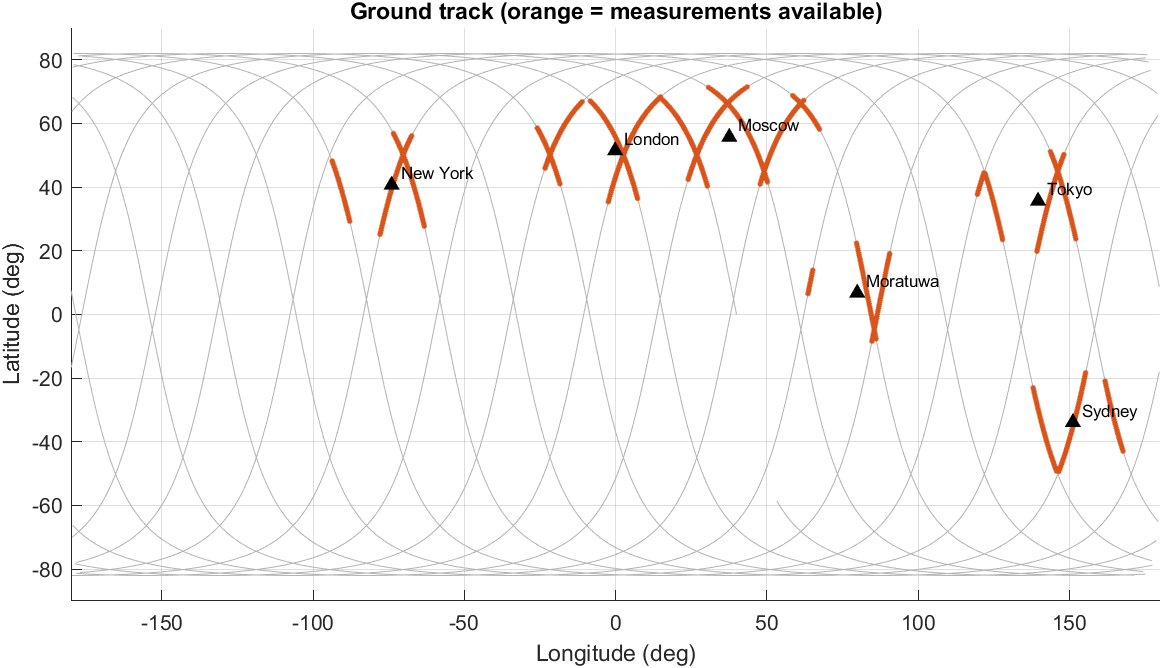
\includegraphics[width=0.88\linewidth]{1_ground_track.png}
\caption{Ground track of the satellite over 24 hours and the six ground stations. Orange points mark epochs with at least one measurement.}
\label{fig:track}
\end{figure}

\paragraph{Estimation error.}
Figure~\ref{fig:errnorm} shows the size of the position and velocity error together with the filter's own one-sigma estimate (the root-sum-square of the diagonal of $\bP$), on a logarithmic scale. The grey bands are the passes.
The filter starts with a 549~m position error and a 2.7~m/s velocity error. The first measurements arrive only after 0.18~h (11 minutes), and by then the velocity error has pushed the position error up to 1.2~km. At the end of the first pass (0.18--0.31~h) the position error is 2.2~m and the velocity error is 5.3~mm/s. The error then grows during the gap that follows (43~m after one hour, and about 70~m just before the second pass) and is pulled down to 0.5~m at the end of the second pass (1.78--1.93~h). After the 2-hour start-up period the error never exceeds 11.9~m in position or 13.2~mm/s in velocity.
The typical saw-tooth shape is clear: the error is pulled down at every pass and then grows slowly during the gaps, because the unmodelled drag and the remaining estimation error are propagated forward without correction. The filter's estimate of its own uncertainty follows the same pattern, mostly slightly above the actual error.

\begin{figure}[!htbp]
\centering
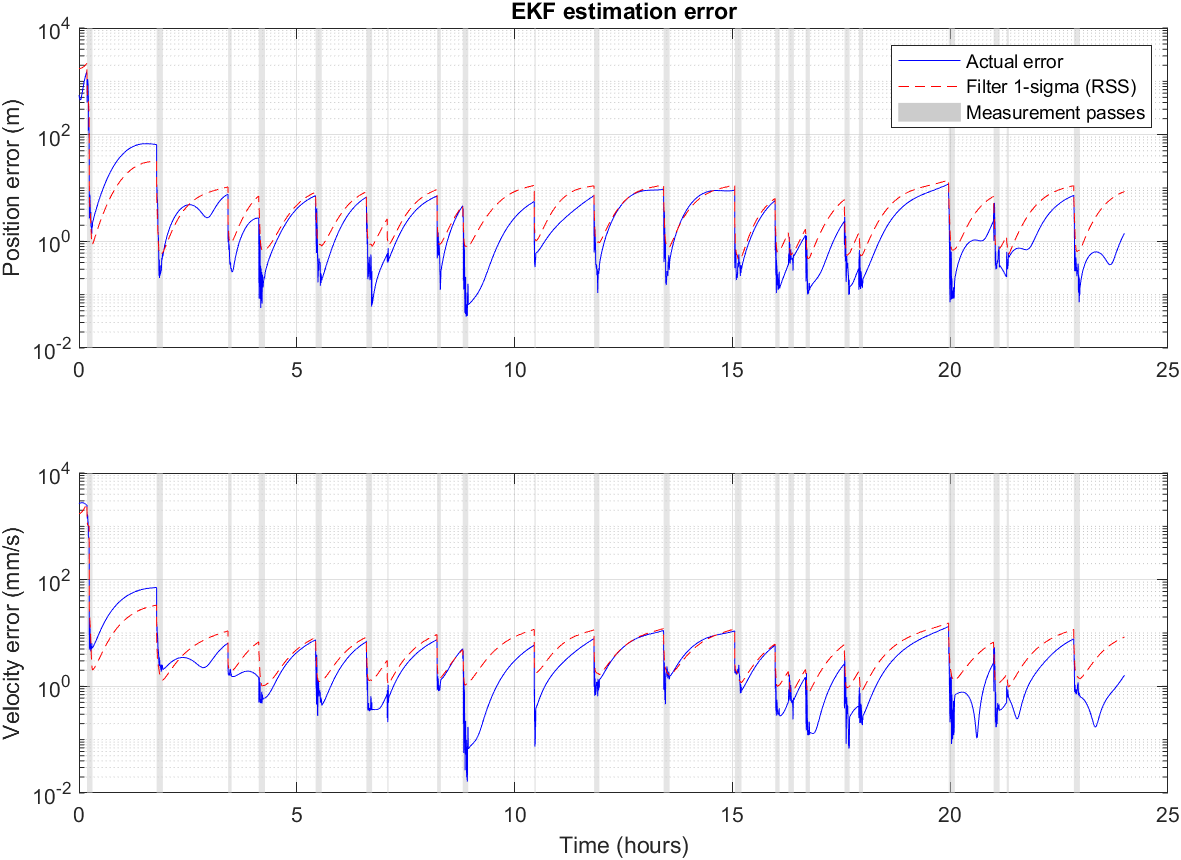
\includegraphics[width=0.88\linewidth]{2_error_norms.png}
\caption{Position error (top) and velocity error (bottom) of the EKF compared with the filter's own one-sigma uncertainty. Grey bands are measurement passes.}
\label{fig:errnorm}
\end{figure}

Table~\ref{tab:baseline} gives the main numbers.

\begin{table}[H]
\centering
\caption{Baseline results (seed 1). RMS, median and maximum values are computed after the first 2 hours.}
\label{tab:baseline}
\begin{tabular}{lcc}
\toprule
\textbf{Quantity} & \textbf{Position} & \textbf{Velocity} \\
\midrule
Initial error & 549~m & 2.69~m/s \\
Error at the end of the first pass (0.31 h) & 2.24~m & 5.25~mm/s \\
Position error after 1 hour & 42.9~m & -- \\
RMS error & 4.03~m & 4.25~mm/s \\
Median error & 1.82~m & -- \\
Maximum error & 11.90~m & 13.22~mm/s \\
Final error (24 h) & 1.42~m & 1.61~mm/s \\
Share of errors inside $\pm3\sigma$ (each state) & 100\% & 100\% \\
\bottomrule
\end{tabular}
\end{table}

Figure~\ref{fig:comp} zooms in on the three position components with their $\pm3\sigma$ bounds after the start-up phase. All errors stay well inside the bounds. The bounds are widest between passes, and they collapse each time new measurements arrive, so the filter correctly reports that it is least certain when it has gone longest without data. The $z$ bounds are somewhat wider than the $x$ and $y$ bounds (on average $\pm8.6$~m against $\pm7.1$~m and $\pm6.3$~m).

\begin{figure}[!htbp]
\centering
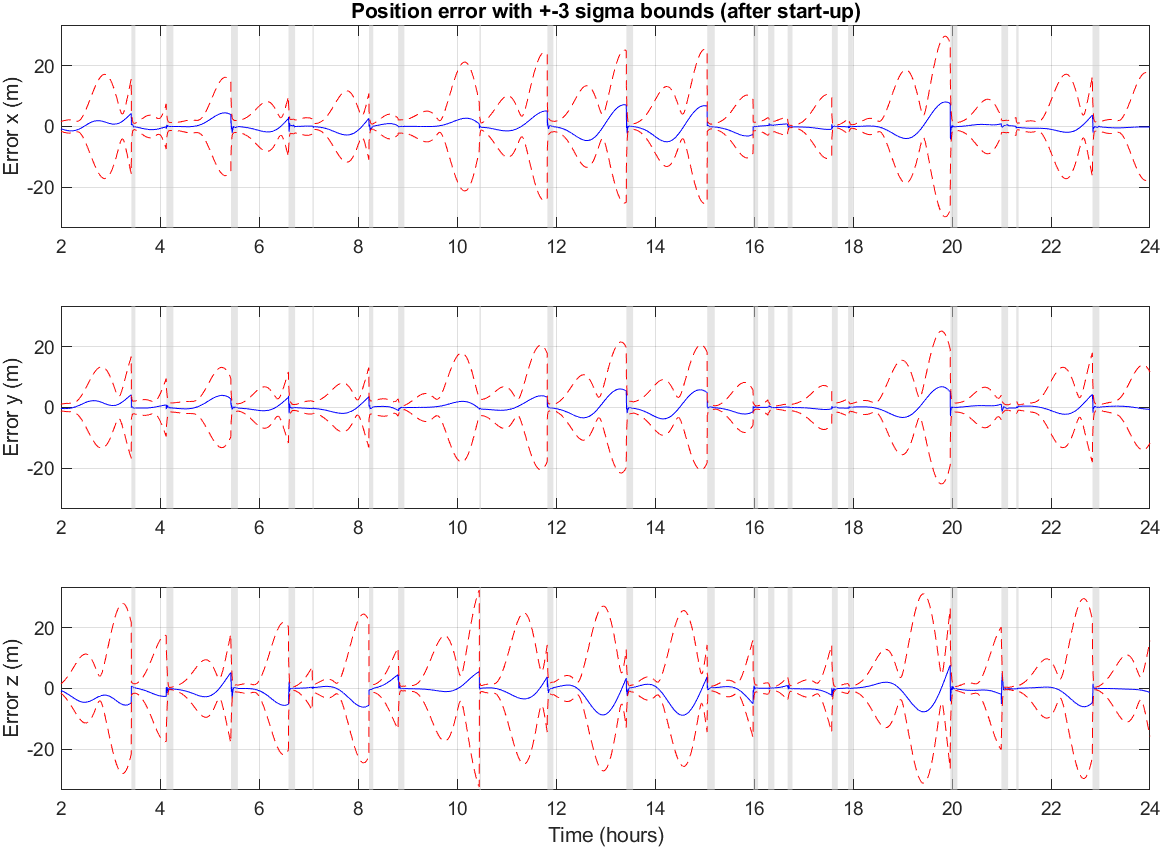
\includegraphics[width=0.88\linewidth]{3_position_components.png}
\caption{Position errors in the three inertial axes (blue) and the $\pm3\sigma$ bounds from the filter covariance (red dashed), after the 2-hour start-up phase.}
\label{fig:comp}
\end{figure}

\paragraph{Innovations.}
Figure~\ref{fig:innov} shows the innovations divided by their predicted standard deviation. They are scattered around zero with unit spread: the mean is $-0.02$ for both range and range-rate, and the standard deviation is 1.00 and 1.03. Only 0.64\% (range) and 0.32\% (range-rate) lie outside $\pm3$, close to the 0.27\% expected for a Gaussian. There is no visible bias for any station, which indicates that the measurement model and the station geometry are correct.

\begin{figure}[!htbp]
\centering
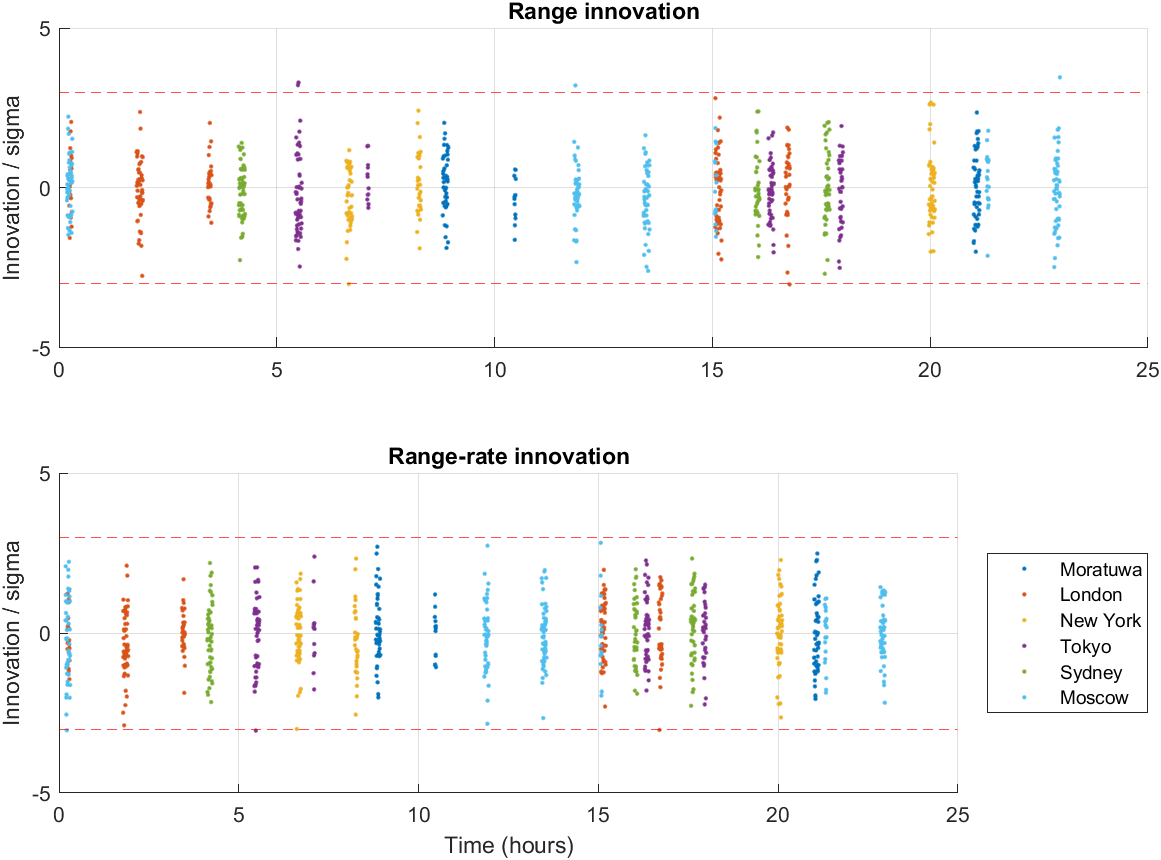
\includegraphics[width=0.88\linewidth]{4_innovations.png}
\caption{Normalised innovations for range (top) and range-rate (bottom), coloured by station. Dashed lines mark $\pm3$.}
\label{fig:innov}
\end{figure}

\paragraph{Consistency.}
Figure~\ref{fig:cons} shows the NEES and NIS. The mean NIS is 2.07 against the ideal value of 2, and 94.3\% of the NIS values fall inside the 95\% bounds (the expected value is 95\%). The per-station mean NIS values lie between 1.90 and 2.18. The innovation statistics are therefore very close to theory.
The mean NEES is 1.74, below the ideal value of 6, and only 50.2\% of NEES values are inside the 95\% bounds: 49.5\% are below the lower bound and only 0.3\% are above the upper bound. This means the filter is conservative: its covariance is somewhat larger than the true error. This is the safer direction (it is consistent with 100\% of the errors lying inside $3\sigma$) and it is caused by a deliberately generous $q$, as explained in Section~\ref{sec:qstudy}.

\begin{figure}[!htbp]
\centering
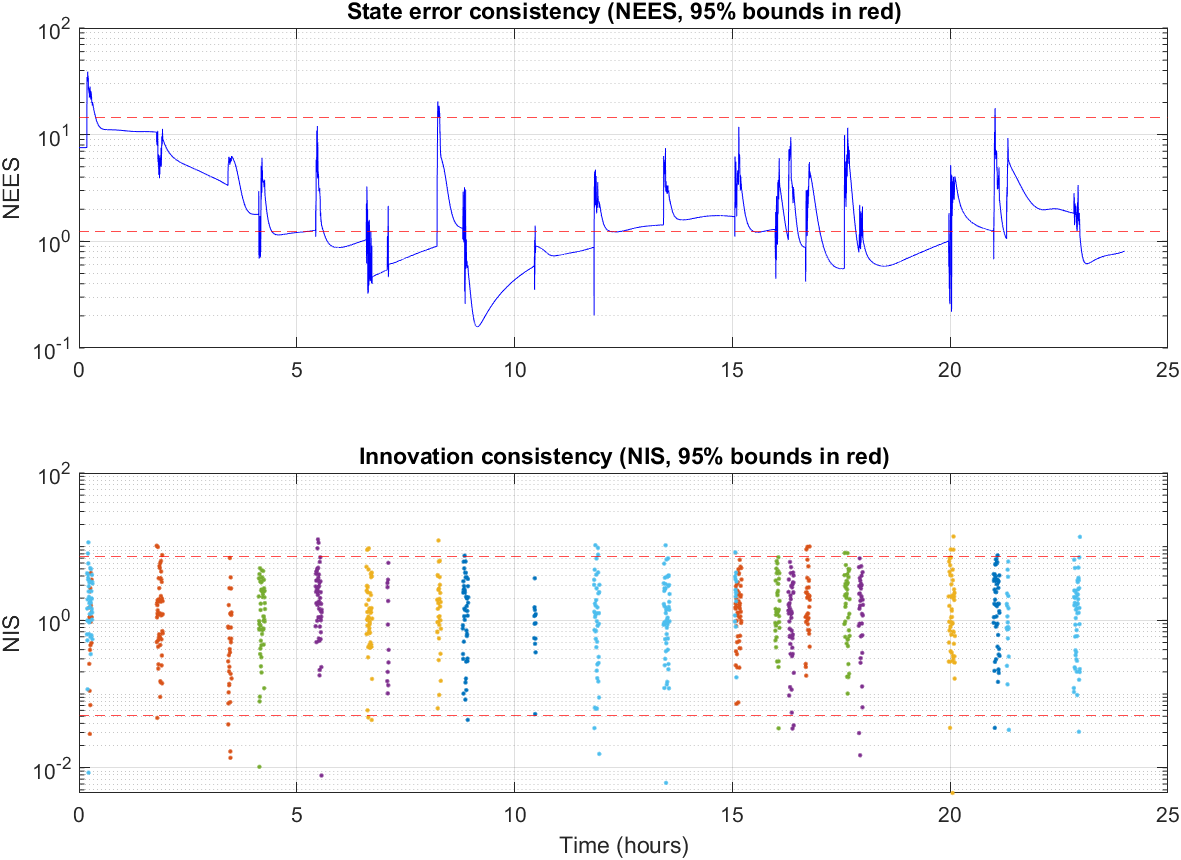
\includegraphics[width=0.88\linewidth]{5_consistency.png}
\caption{NEES (top) and NIS (bottom) with 95\% chi-square bounds (red dashed). Different NIS colours are different stations.}
\label{fig:cons}
\end{figure}

\subsection{Visualisation of the simulation}
To make the scenario easier to understand, the simulation can also be played as a 3D animation (\texttt{run\_animation.m}, which uses \texttt{animate\_orbit.m}). A recorded video, \texttt{orbit\_animation.mp4}, is included with the submitted files.
The animation shows the rotating Earth, the six stations (yellow triangles), the true satellite (yellow dot) with its last orbit as a white trail, the EKF estimate (red ring), a green line of sight for each station that is currently tracking, and, on the right, the position error curve filling in as time passes. Because the estimation error is a few metres and the orbit radius is 7000~km, the red ring sits exactly on top of the yellow dot at this scale; the error panel shows the difference.
Figures~\ref{fig:anim1}--\ref{fig:anim3} show three snapshots.

\begin{figure}[!htbp]
\centering
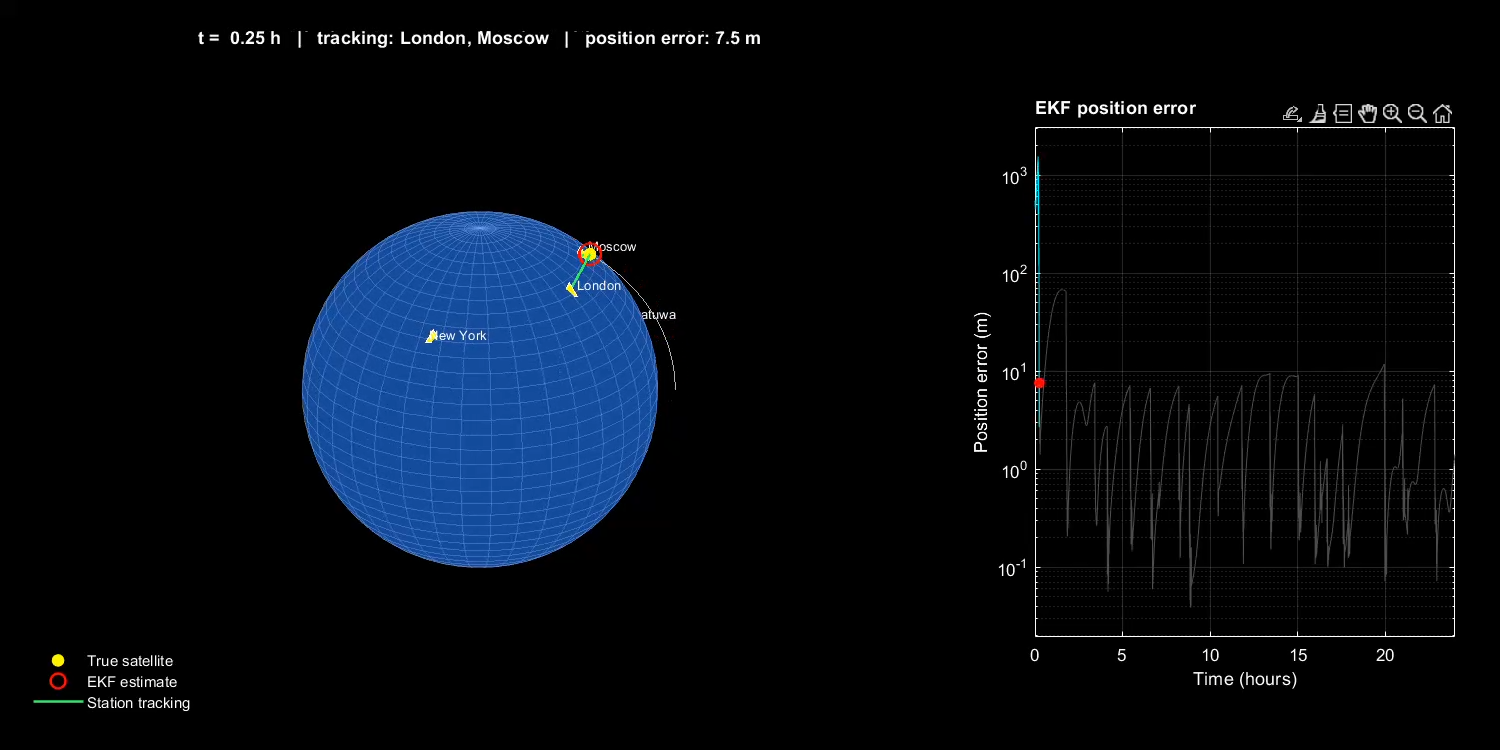
\includegraphics[width=0.88\linewidth]{7_animation_frame_1.png}
\caption{Animation snapshot at $t=0.25$~h, during the first pass: London and Moscow are both tracking the satellite and the error is falling quickly (7.5~m).}
\label{fig:anim1}
\end{figure}

\begin{figure}[!htbp]
\centering
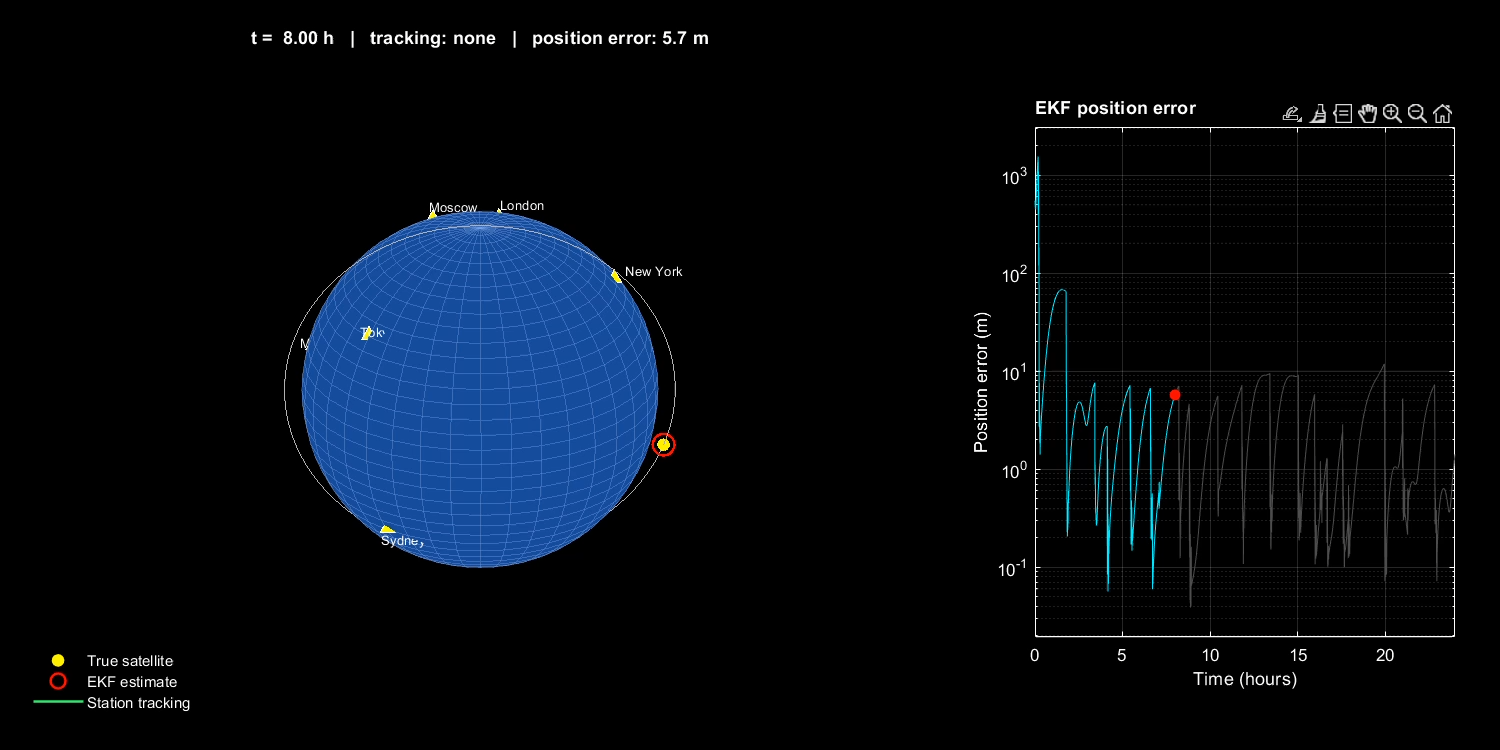
\includegraphics[width=0.88\linewidth]{7_animation_frame_3.png}
\caption{Animation snapshot at $t=8.0$~h, in a gap between passes: no station sees the satellite, so the filter is only predicting and the error (5.7~m) is slowly growing.}
\label{fig:anim2}
\end{figure}

\begin{figure}[!htbp]
\centering
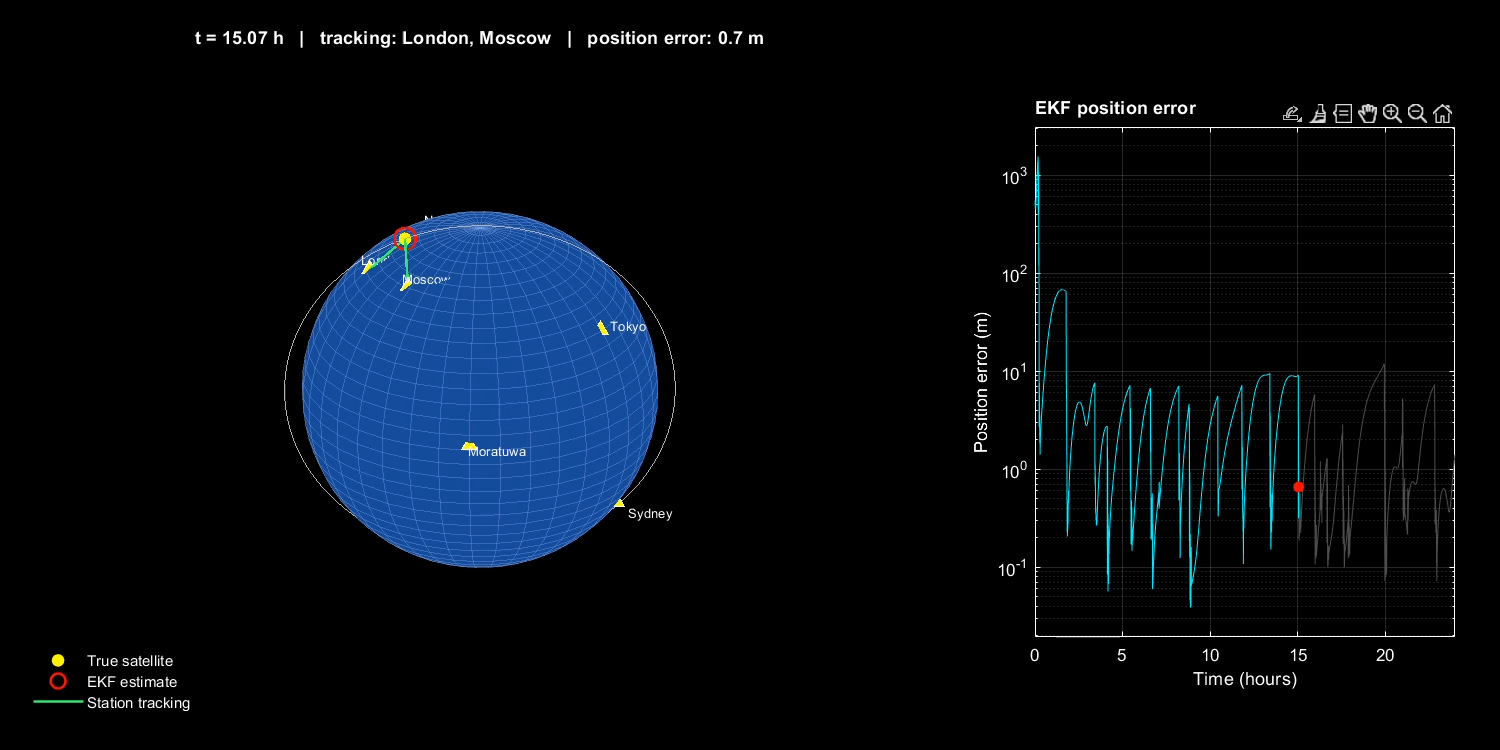
\includegraphics[width=0.88\linewidth]{7_animation_frame_2.png}
\caption{Animation snapshot at $t=15.1$~h: London and Moscow are tracking again and the error has been pulled back down to 0.7~m. The cyan curve on the right shows the error history so far.}
\label{fig:anim3}
\end{figure}

\subsection{Parameter studies}
Each study below changes one setting from the baseline and reports the RMS position error after the 2-hour start-up period. They were produced by \texttt{run\_experiments.m}, and a summary is shown in Figure~\ref{fig:studies}. Each case uses a single random seed unless stated otherwise. ``Diverged'' means that the RMS error is of the order of the orbit radius or larger.

\subsubsection{Monte Carlo test}
To check that the baseline result is not a lucky seed, the baseline was repeated for 20 seeds, which changes the measurement noise and the initial error. The RMS position error was $3.78\pm0.33$~m (mean $\pm$ standard deviation over runs) and the mean NEES was 1.68. None of the 20 runs diverged.

\subsubsection{Number of ground stations}
\begin{table}[H]
\centering
\caption{Effect of the number of stations (stations are added in the order shown).}
\label{tab:stations}
\begin{tabular}{clccc}
\toprule
\textbf{Stations} & \textbf{Added station} & \textbf{Passes} & \textbf{Longest gap (h)} & \textbf{RMS position error (m)} \\
\midrule
1 & Moratuwa  & 3  & 10.5 & diverged ($4.6\times10^{7}$) \\
2 & London    & 8  & 5.3  & 38.1 \\
3 & New York  & 11 & 4.6  & 891 \\
4 & Tokyo     & 15 & 4.6  & 6235 \\
5 & Sydney    & 18 & 4.6  & 291 \\
6 & Moscow    & 22 & 2.0  & 4.03 \\
\bottomrule
\end{tabular}
\end{table}
A single station is not enough: the filter diverges. With all six stations the filter works very well (4.0~m). The cases with three to five stations are much worse (about 290 to 6200~m RMS), although the filter does not stay lost: over the last six hours the RMS error is 50~m (3 stations), 25~m (4 stations) and 5.8~m (5 stations). Their large errors come from the first part of the run. With three to five stations the longest gap between passes is 4.6~hours, and during this gap the error grows to kilometres (maximum error after the start-up phase: 4.1~km, 31.8~km and 1.5~km for 3, 4 and 5 stations, against 11.9~m for six stations). An error of that size is close to the limit where the EKF linearisation stops being valid (see the initial-error study below), so the filter recovers only slowly.
The gap length does not explain everything, because the two-station case has an even longer gap (5.3~h) but a smaller error (38~m). The quality of the orbit estimate at the end of each pass, which depends on the geometry of that pass, also matters. With a single seed the ordering of the three-, four- and five-station cases should therefore not be over-interpreted; the clear conclusion is that frequent passes (six stations, longest gap 2.0~h) keep the filter accurate.

\subsubsection{Process noise}
\label{sec:qstudy}
\begin{table}[H]
\centering
\caption{Effect of the process-noise level $q$.}
\label{tab:q}
\begin{tabular}{ccc}
\toprule
$q$ (km$^2$/s$^3$) & \textbf{RMS position error (m)} & \textbf{Mean NEES} \\
\midrule
$10^{-18}$ & 3.91 & 48.81 \\
$10^{-17}$ & 3.67 & 6.34 \\
$10^{-16}$ (baseline) & 4.03 & 1.74 \\
$10^{-15}$ & 4.94 & 0.78 \\
$10^{-14}$ & 5.68 & 0.41 \\
$10^{-13}$ & 14.30 & 0.41 \\
\bottomrule
\end{tabular}
\end{table}
This is a classical tuning trade-off. If $q$ is too small ($10^{-18}$), the filter becomes overconfident (NEES $=49$), because it trusts its dynamics model too much and gives too little weight to the measurements. If $q$ is too large ($10^{-13}$), the filter gives too much weight to noisy measurements, the error grows (14~m) and the NEES drops to 0.4. The RMS error is lowest at $q=10^{-17}$ (3.7~m) and stays below 6~m up to $10^{-14}$.
The NEES is closest to its ideal value of 6 at $q=10^{-17}$, but this value has little margin: a slightly different disturbance would make the filter overconfident. The baseline uses $q=10^{-16}$, which gives nearly the same accuracy (4.0~m) with a safety margin, at the price of a conservative covariance.

\subsubsection{Initial error}
\begin{table}[H]
\centering
\caption{Effect of the initial position error (the initial velocity error is $10^{-3}$ times this value in km/s, and $\bP_0$ is scaled to match).}
\label{tab:init}
\begin{tabular}{cc}
\toprule
\textbf{Initial position error (km)} & \textbf{RMS position error (m)} \\
\midrule
0.1 & 3.93 \\
1 (baseline) & 4.03 \\
5 & 12.23 \\
20 & 270.4 \\
50 & diverged ($2.0\times10^{7}$) \\
100 & diverged ($1.1\times10^{11}$) \\
\bottomrule
\end{tabular}
\end{table}
The filter is insensitive to the initial error up to a few kilometres, degrades noticeably at 20~km and diverges at 50~km. This is the main limitation of the EKF: it linearises about its current estimate, and when that estimate is far from the truth the Jacobians describe the wrong point of the nonlinear model, so corrections can push the estimate in the wrong direction and the filter can never recover.

\subsubsection{Measurement noise}
\begin{table}[H]
\centering
\caption{Effect of the measurement noise (multiplier on both $\sigma_\rho=10$~m and $\sigma_{\dot\rho}=1$~mm/s; the filter's $\bR$ is changed to match).}
\label{tab:noise}
\begin{tabular}{cc}
\toprule
\textbf{Noise multiplier} & \textbf{RMS position error (m)} \\
\midrule
0.1 & 3.04 \\
1 (baseline) & 4.03 \\
5 & 4.84 \\
10 & 6.13 \\
\bottomrule
\end{tabular}
\end{table}
Increasing the measurement noise by a factor of 10 increases the error by only about 50\%. The accuracy is therefore not limited mainly by the quality of each individual measurement. A likely explanation is that each pass contains tens of epochs whose noise averages out, so that the accuracy is dominated by the growth of the error between passes due to unmodelled forces.

\subsubsection{Dynamics model: the role of \texorpdfstring{$J_2$}{J2}}
\label{sec:j2study}
When the filter uses only two-body gravity, but the truth still contains $J_2$, the filter diverges completely (RMS error $9.1\times10^{6}$~m), even though $q$ was increased to $10^{-9}$~km$^2$/s$^3$ to compensate. The reason is that the $J_2$ error accumulates as a large, systematic along-track drift of the order of 150~km over one typical gap between passes (Section~\ref{sec:dyn}). That is far outside the range where the EKF linearisation is valid (compare the initial-error study) and it is not white noise, so adding process noise cannot fix it. A good dynamics model is more valuable than a large $q$.

\begin{figure}[!htbp]
\centering
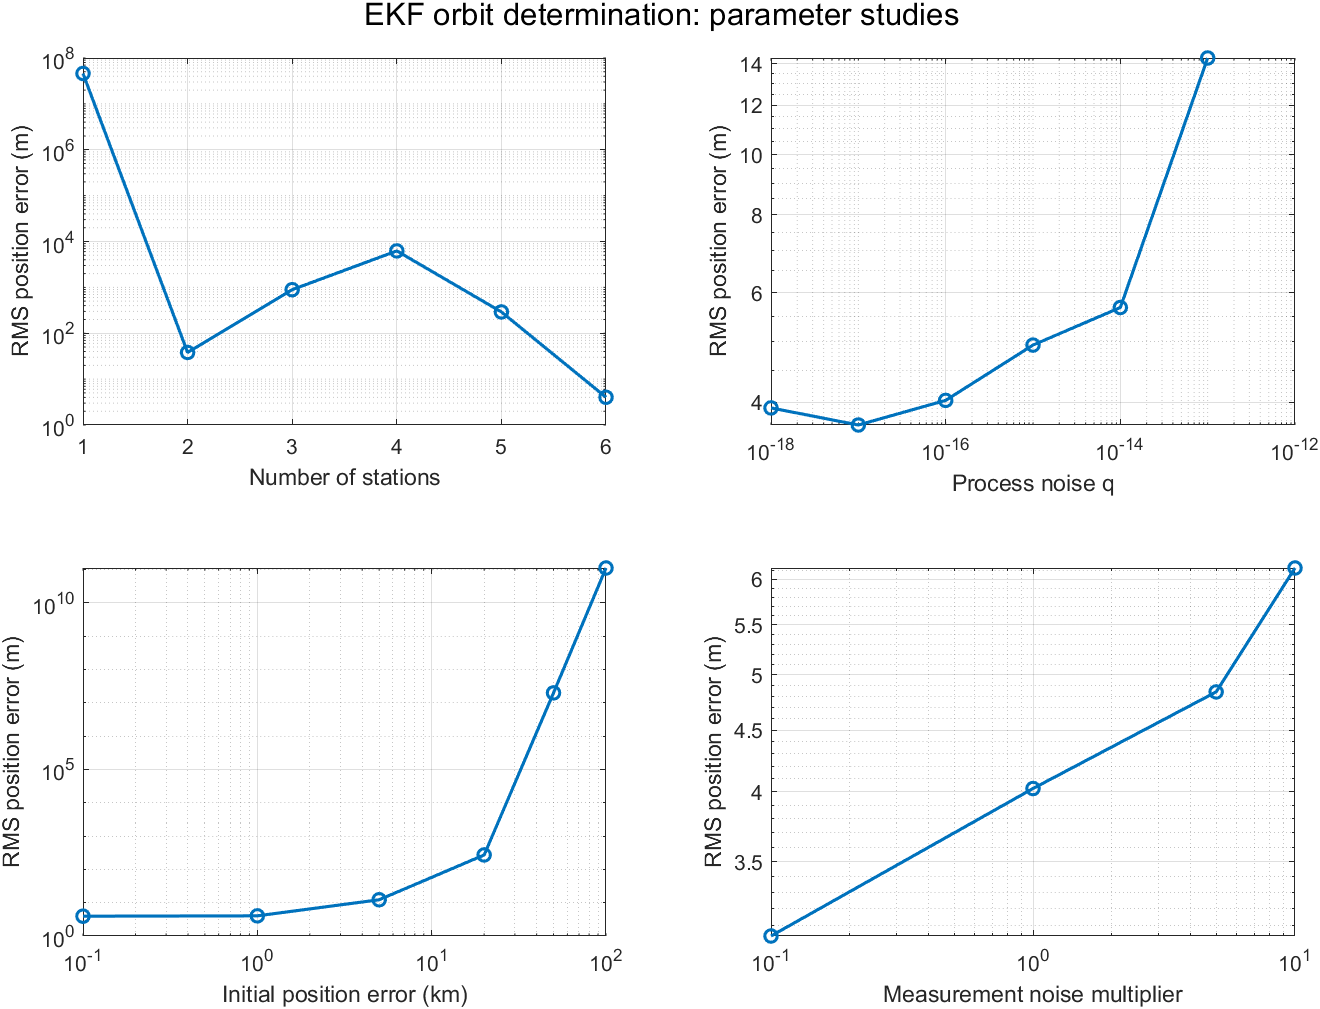
\includegraphics[width=0.88\linewidth]{6_parameter_studies.png}
\caption{Parameter studies: RMS position error versus number of stations, process noise, initial position error and measurement noise multiplier.}
\label{fig:studies}
\end{figure}

% ==================================================================
% 5 Discussion
% ==================================================================
\clearpage
\section{Discussion}

\paragraph{Effectiveness of the EKF.}
For the baseline scenario the EKF is very effective. It brings the position error from 549~m (and a 2.7~m/s velocity error) down to a few metres after the very first pass, after the first two hours it keeps the error below 12~m, and it does so while being able to see the satellite for only 10.5\% of the time. Both the innovation statistics and the $3\sigma$ coverage show the filter is well calibrated. It is also very cheap: a full 24-hour run takes 0.6~s on a laptop.

\paragraph{Why the accuracy is limited by the gaps and not the sensors.}
The results show a clear pattern: the error is small right after each pass and grows between passes (Figure~\ref{fig:errnorm}), and the accuracy barely depends on the measurement noise (Table~\ref{tab:noise}). A bigger improvement could therefore be gained from better force modelling (for example estimating the drag coefficient as an extra state) than from better ranging hardware.

\paragraph{Observability and the number of stations.}
Each epoch delivers only two numbers (a distance and its rate of change) for a six-dimensional state, so the full state must be reconstructed from how the range and Doppler curves change over a pass and from many passes. With a single station and a sparse pass schedule (three passes in 24 hours, longest gap 10.5~hours) the information appears to be insufficient and the filter diverges. With three to five stations the filter suffers from long gaps of 4.6~hours, and only with six stations does the longest gap fall to 2.0~hours and the error stay at a few metres (Table~\ref{tab:stations}). More stations therefore help mainly by making the passes frequent enough to keep the error in the region where the linearisation holds.

\paragraph{Limits of the EKF.}
The EKF is a sub-optimal estimator, because it replaces the nonlinear models with linear approximations, and its Kalman gain is only near-optimal. The studies show three situations where this approximation breaks down or struggles: a large initial error (50~km or more), an incomplete dynamics model ($J_2$ left out), and too little data (one station, or long gaps). In all of them the cause is the same: the filter linearises about an estimate that is too far from the truth. Possible remedies include an iterated EKF (re-linearising the correction step), an unscented Kalman filter, or using a batch least-squares fit of the first passes to obtain a better initial state before switching to the EKF. A particle filter would also be robust against large initial errors but would be much more expensive.

\paragraph{Tuning and conservatism.}
The process noise had a large effect. A value that is too small gives overconfident (inconsistent) estimates and a value that is too large gives noisier ones. The baseline $q$ is slightly conservative, so the NEES is below its ideal value, but the real error is always within $3\sigma$ and the NIS is almost exactly 2. For an operational system, a conservative covariance is usually preferred to an overconfident one.

\paragraph{Limitations of this study.}
\begin{itemize}
  \item The results come from simulation. The truth model is simpler than reality (constant drag, no third-body forces or solar pressure, no precession or nutation, no measurement biases or atmospheric delays), so the absolute error values should not be compared with real tracking systems.
  \item The stations are treated as ideal range and Doppler sensors with the same noise at every location, and the station locations are only used as convenient, well-known positions on the globe.
  \item The parameter studies use one seed per case (except the Monte Carlo test), so small differences, such as among the three-, four- and five-station cases, are not statistically proven.
  \item The tracked satellite is in a single orbit; eccentric or higher-altitude orbits were not tested.
\end{itemize}

% ==================================================================
% 6 Conclusion
% ==================================================================
\clearpage
\section{Conclusion}
An Extended Kalman Filter for satellite orbit determination from ground-station range and range-rate measurements was derived, implemented in MATLAB and evaluated in a 24-hour simulation with six stations (Moratuwa, London, New York, Tokyo, Sydney and Moscow).
The measurement Jacobian was derived analytically, and the state-transition matrix was obtained by integrating the variational equations of a two-body $+\,J_2$ model.
In the baseline scenario the filter reduced an initial error of 549~m and 2.7~m/s to an RMS error of 4.0~m in position and 4.3~mm/s in velocity, with measurements available only 10.5\% of the time, and the NIS, normalised-innovation and $3\sigma$ tests showed that the filter is consistent. A Monte Carlo test over 20 runs confirmed this ($3.78\pm0.33$~m). A 3D animation of the satellite, the stations and the tracking lines was also produced to illustrate the scenario.
The parameter studies showed that the accuracy depends strongly on the number and geometry of the stations (through the length of the gaps between passes), on correct tuning of the process noise and on including $J_2$ in the model, and only weakly on the measurement noise. They also showed the main weakness of the EKF: it diverges when the initial error is too large (about 50~km), when there is too little data (one station) or when the model is wrong.
Future work could estimate the drag coefficient as an additional state, compare the EKF with an unscented Kalman filter and with batch least squares, and use real tracking data.

% ==================================================================
% Appendix
% ==================================================================
\appendix
\clearpage
\section{MATLAB code}
The listings below are the complete core code. To reproduce the results, put all files in one folder, run \texttt{run\_orbit\_ekf} for the baseline scenario and \texttt{run\_experiments} for the parameter studies. To play the 3D animation, run \texttt{run\_animation}. The plotting and printing helpers (\texttt{plot\_results.m}, \texttt{print\_summary.m}) are submitted with the code but are not listed here.

\Needspace*{22\baselineskip}
\subsection{Main script}
\lstinputlisting[caption={\texttt{run\_orbit\_ekf.m}}]{code/run_orbit_ekf.m}

\Needspace*{56\baselineskip}
\subsection{Configuration}
\lstinputlisting[caption={\texttt{default\_config.m}}]{code/default_config.m}

\Needspace*{35\baselineskip}
\subsection{Simulation}
\lstinputlisting[caption={\texttt{run\_simulation.m}}]{code/run_simulation.m}
\Needspace*{20\baselineskip}
\lstinputlisting[caption={\texttt{simulate\_truth.m}}]{code/simulate_truth.m}
\Needspace*{32\baselineskip}
\lstinputlisting[caption={\texttt{simulate\_measurements.m}}]{code/simulate_measurements.m}
\Needspace*{27\baselineskip}
\lstinputlisting[caption={\texttt{kepler\_to\_state.m}}]{code/kepler_to_state.m}
\Needspace*{26\baselineskip}
\lstinputlisting[caption={\texttt{station\_eci.m}}]{code/station_eci.m}

\Needspace*{22\baselineskip}
\subsection{Dynamics and measurement models}
\lstinputlisting[caption={\texttt{orbit\_accel.m}}]{code/orbit_accel.m}
\Needspace*{47\baselineskip}
\lstinputlisting[caption={\texttt{propagate\_state.m}}]{code/propagate_state.m}
\Needspace*{19\baselineskip}
\lstinputlisting[caption={\texttt{range\_model.m}}]{code/range_model.m}

\Needspace*{23\baselineskip}
\subsection{Extended Kalman Filter}
\lstinputlisting[caption={\texttt{ekf\_predict.m}}]{code/ekf_predict.m}
\Needspace*{20\baselineskip}
\lstinputlisting[caption={\texttt{ekf\_update.m}}]{code/ekf_update.m}
\Needspace*{46\baselineskip}
\lstinputlisting[caption={\texttt{run\_ekf.m}}]{code/run_ekf.m}

\Needspace*{40\baselineskip}
\subsection{Parameter studies}
\lstinputlisting[caption={\texttt{run\_experiments.m}}]{code/run_experiments.m}

\Needspace*{22\baselineskip}
\subsection{3D animation}
\lstinputlisting[caption={\texttt{run\_animation.m}}]{code/run_animation.m}
\Needspace*{40\baselineskip}
\lstinputlisting[caption={\texttt{animate\_orbit.m}}]{code/animate_orbit.m}

\end{document}
